\documentclass[a4paper, 12pt]{article}
\usepackage{fontspec}
\setmainfont{Arial}
\usepackage[margin=2.0cm]{geometry}
\usepackage{wrapfig}

\author{Dr Luke Hindson}
\title{\vspace{-1.45cm}VocaLink: Wikipedia Analysis
\date{}
}
 
\begin{document}
\maketitle
\vspace{-10pt}

\noindent The Wikipedia statistics page\footnote{https://en.wikipedia.org/wiki/Wikipedia:Statistics} indicates that there are over 10 edits to Wikipedia pages per second. Information regarding these edits can potentially provide a powerful insight into current trends and events in the world. Below I explore two potential applications.

\subsection*{Visualisation: 1}

\textbf{Question: Within a given time frame what are the most popular types of pages being edited on Wikipedia?}

\noindent This may seem like a simple question but it has the potential to highlight trends in current events. There are a number of ways we could present the most popular edit topics. One of the most intuitive and easy to grasp is a word cloud, whereby frequent words appear large whilst less frequent words appear small. The downside of this approach is that it does not provide any information as to the actual frequency of words. Nevertheless, word clouds are often useful as a first look or for less quantitatively rigorous presentations.  In Fig.~\ref{im:1} I present a word cloud of the 100 most frequent words taken from the titles of Wikipedia edits over a 24\,hr period. It is immediately apparent that topics including the United States, sports teams, and New York are popular. This provides a jumping off point for further questions. There are a number of improvements that could be made. The most obvious is applying a more rigorous approach to identifying the primary words of a title or page.  Natural Language Processing would be a useful tool for this. 

\begin{figure*}[h]
\begin{center}
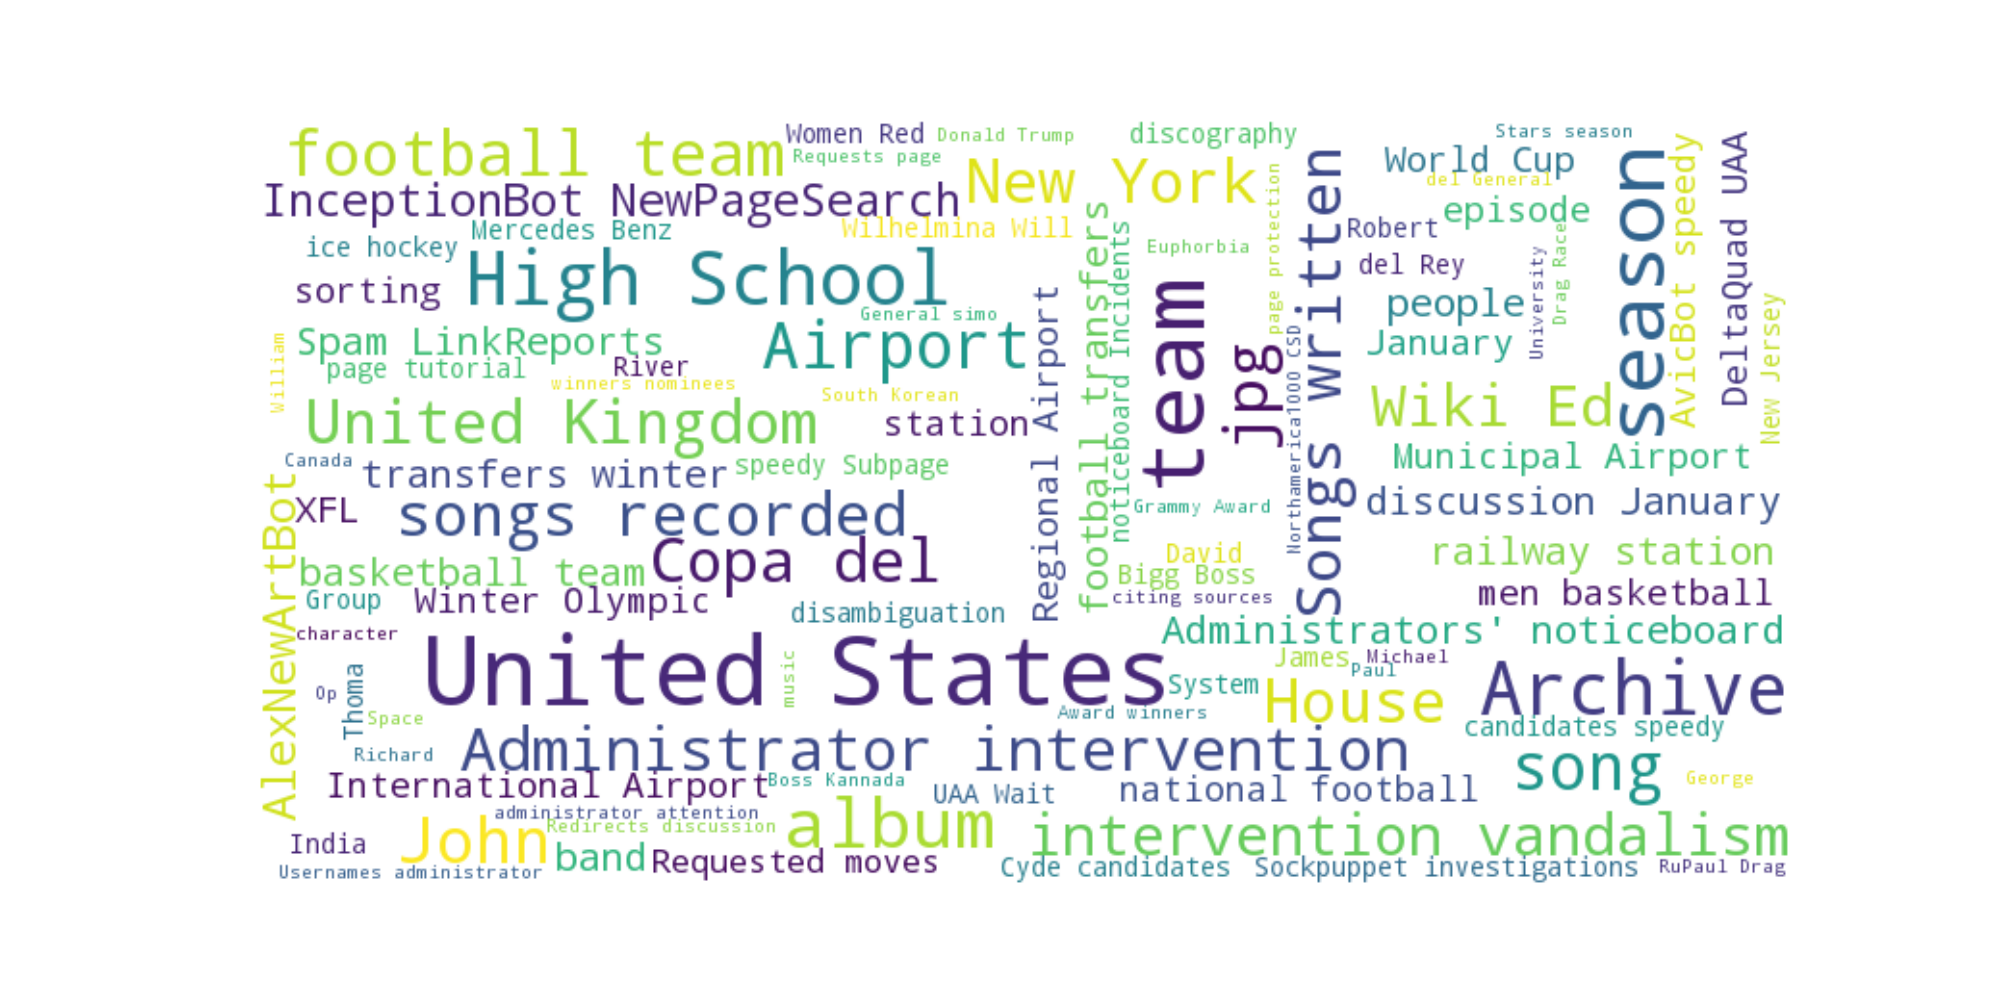
\includegraphics[width=0.9\textwidth, trim={3cm 3cm 3cm 3cm},clip]{./IMAGES/wordcloud.png} 
\caption{Word cloud results for a 24\,hr period.}
\label{im:1}
\end{center}
\end{figure*}

\newpage
\subsection*{Visualisation: 2}

\textbf{Question: Can we identify the source of malicious edits?}

\noindent The open source nature of Wikipedia is one of its greatest strengths but makes the platform open to exploitation. Wikipedia uses an AbuseFilter to prevent patterns of harmful editing. It would be interesting to identify where the majority of these harmful edits come from. People or bots that edit Wikipedia entries often remain anonymous or can easily fake their locations. A comparison of time against AbuseFilter hit frequency may be informative. Countries where abuse is more frequent are likely to be seen as a spike at times when the local population is awake. This behaviour may also be seen in the number of known and unknown locations for edits under the assumption that more abusive editors will hide their location leading to rise in the fraction of edits with unknown locations. 
\\
\\
\noindent In the top panel of Fig.~\ref{im:2} I show the number of edits that were logged as ``AbuseFilter'' in a 24\,hr period in bins of 30\,mins. In the bottom panel of this figure the fraction of edits coming from unknown locations is shown for each time bin. The mean (dashed blue-line), rolling mean (solid blue-line), and rolling standard deviation (solid red-line) are shown. This plot clearly shows an increase in the frequency of abuse after 15:00 GMT. The fraction of unknown locations appears fairly constant. Further data needs to be gathered to confirm this trend but it would appear that malicious edit frequency increases after 15:00 GMT.

\begin{figure*}[h]
\begin{center}
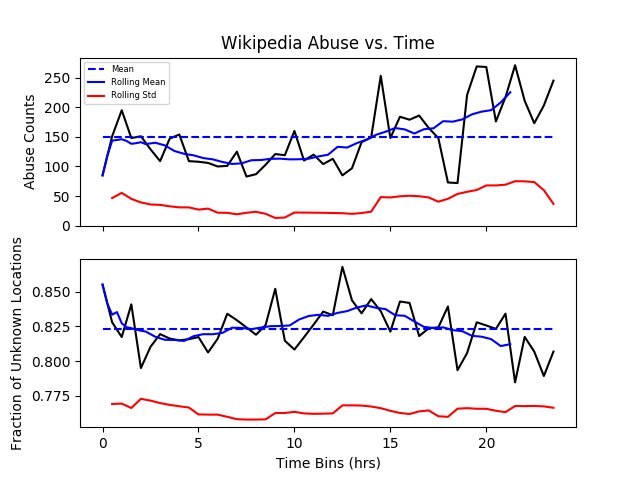
\includegraphics[width=0.9\textwidth]{./IMAGES/abuse.png} 
\caption{Top: plot of time and abuse log counts. Bottom: fraction of edits from unknown locations.}
\label{im:2}
\end{center}
\end{figure*}


\end{document}
